\documentclass[problem]{mcs}

\begin{pcomments}
    \pcomment{TP_The_Divisibility_DAG}
    \pcomment{Converted from divides-dag.scm
              by scmtotex and dmj
              on Sun 13 Jun 2010 02:58:06 PM EDT}
\pcomment{modified 28 july 2011 by drewe}
\end{pcomments}

\begin{problem}

%% type: short-answer
%% title: The Divisibility DAG

In this DAG (Figure ~\ref{fig:divi2}) for the divisibility relation on
$\set{1, \dots, 12}$, there is an upward path from $a$ to~$b$ iff $a
\divides b$.  If 24 was added as a vertex, what is the minimum number
of edges that must be added to the DAG to represent divisibility on
$set{1, \dots, 12, 24}$?  What are those edges?

\begin{center}
\begin{figure}[h!]
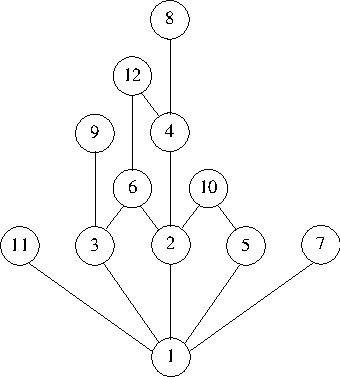
\includegraphics[height=35mm]{../figures/drafts/divi2.pdf}
\caption{\label{fig:divi2}}
\end{figure}
\end{center}

\begin{solution}
2

Edges from 8 and 12 to 24 are all that are needed.
\end{solution}

\end{problem}

\endinput
